\section*{Краткое описание предметной области}
Настольная игра -- игра, основанная на манипуляции относительно небольшим набором предметов, которые могут целиком разместиться на столе или в руках играющих.

Целевой аудиторией проекта являются люди от 12 лет, которым нравятся настольные игры. В магазинах сети для которой разрабатывается проект, продаются игры как долгие и сложные игры для группы не больше четырех человек, так и простые игры для большой компании.

Настольные игры подлежат обязательной сертификации согласно стандарту ТР ТС 008/2011 <<О безопасности игрушек>>. 

Для того чтобы пользователь не искал по магазинам сети, где интересующая его настольная игра есть в наличии необходимо создать портал который будет агрегировать все настольные игры во всех магазинах данной сети. 

Для предотвращения выкупа настольной игры другим клиентом игра может быть забронирована на неделю. В течение этого времени клиент может оставить заявку на отказ от бронирования. 

Необходимо предусмотреть, что покупатель может прийти в магазин и купить игру без предварительного бронирования.

Данное техническое задание определяет требования к разработке интеграционного портала для поиска и бронирования настольной игры в магазинах настольных игр.


\section*{Существующие аналоги}

Среди аналогов можно такой интернет-магазин как <<Игровед>>\\ (www.igroved.ru). Он позволяет искать и покупать настольные игры в магазинах их сети, но он не реализует функционал рекомендованного поиска игр. Также существуют такие маркетплейсы как Wildberries \\(www.wildberries.ru) и Ozon (www.ozon.ru), но за пользование их системой они берут комиссию с продавцов. 

\section*{Основания для разработки}
Разработка ведётся в рамках выполнения лабораторных работ по курсу <<Методология программной инженерии>> на кафедре <<Программное обеспечение ЭВМ и информационные технологии>> факультета <<Информатика и системы управления>> МГТУ им. Н.Э. Баумана.

\section*{Назначение разработки}
Разрабатываемая система должна предоставлять пользователям возможность поиска наличия интересующих их настольных игр в магазинах по продаже настольных игр. Должен быть предусмотрен механизм бронирования настольных игр для предотвращения их покупки другими пользователями

\section*{Описание системы}
Разрабатываемый сервис должен представлять собой распределённую систему для поиска и бронирования настольных игр. Каждый магазин имеет свою базу данных для учета товара.

Система должна обеспечивать разделение пользователей на три роли:
\begin{itemize}
	\item \textbf{пользователь} — неавторизованный пользователь;
	\item \textbf{клиент} — авторизованный пользователь;
	\item \textbf{администратор} -- пользователь ответственный за поддержку Системы.
\end{itemize}

Если \textbf{клиент} хочет оформить бронь, ему необходимо зарегистрироваться, указав информацию: фамилия, имя, электронная почта. В случае, если зарегистрированному ранее пользователю нужно оставить заявку на отмену бронирования или получить информацию о его бронированиях ему нужно авторизоваться.

Для \textbf{неавторизованных пользователей} доступен только поиск настольных игр по магазинам.

Для \textbf{администратора} должен быть предусмотрен функционал изменения наличия настольных игр в магазинах, а также добавление новых магазинов.

\section*{Общие требования к системе}
Требования к системе следующие.
\begin{enumerate}
	\item Разрабатываемое ПО должно поддерживать функционирование системы в режиме 24 часов, 7 дней в неделю, 365 дней в году (24/7/365) со среднегодовым временем доступности не менее 99.9\%. Допустимое время, в течении которого система недоступна, за год должна составлять $24\cdot365\cdot0.001=8.76$ ч.
	
	\item Время восстановления системы после сбоя не должно превышать 15 минут.
	
	\item Каждый узел должен автоматически восстанавливаться после сбоя.
	
	\item Обеспечить безопасность работоспособности за счёт отказоустойчивости узлов.
\end{enumerate}

\section*{Требования к функциональным характеристикам}
\begin{enumerate}
	\item По результатам работы модуля сбора статистики медиана времени отклика системы на запросы пользователя на получение информации не должна превышать 3 секунд.
	
	\item Медиана времени отклика системы на действия пользователя должна быть менее 0.8 секунд при условии работы на рекомендованной аппаратной конфигурации, задержках между взаимодействующими сервисами менее 0.2 секунды и одновременном числе работающих пользователей менее 100 на каждый сервер, обслуживающий внешний интерфейс.
	
	\item Система должна обеспечивать возможность запуска в современных браузерах: не менее 85\% пользователей Интернета должны пользоваться ей без какой-либо деградации функционала.
\end{enumerate}

\section*{Функциональные требования к системе с точки зрения пользователя}

Портал должен обеспечивать реализацию следующих функций:
\begin{enumerate}
    \item Система должна обеспечивать регистрацию пользователей с проверкой правильности вводимых данных.
    \item Система должна обеспечивать аутентификацию пользователей.
    \item Система должна обеспечивать разделение пользователей на три роли.
    \item Система должна предоставлять \textbf{администратору} следующие функции:
    \begin{itemize}
        \item просмотр и изменение списка магазинов, входящих в сеть;
        \item просмотр наличия настольных игр в магазинах сети;
        \item авторизация в системе;
        \item получение изменение детальной информации по конкретному бронированию;
        \item подтверждение оплаты бронирования;
        \item отмена оформленного бронирования по заявке;
    \end{itemize}
    \item Система должна предоставлять \textbf{клиенту} следующие функции:
    \begin{itemize}
        \item просмотр истории бронирований;
        \item бронирование настольной игры в одном из магазинов, где она есть в наличии;
        \item получение, изменение детальной информации по конкретному бронированию;
        \item составление заявки на отмену оформленного заказа.
    \end{itemize}
    \item Система должна предоставлять \textbf{пользователю} следующие функции:
    \begin{itemize}
        \item просмотр информации о магазинах: контакты,  местоположение;
        \item просмотр информации о настольных играх: название, описание, правила игры, наличие в магазинах;
        \item регистрация;
        \item авторизация.
    \end{itemize}
\end{enumerate}



\section*{Входные данные}
Входные параметры системы представлены в таблице 
\begin{enumerate}
    \item Клиент / Администратор 
    \begin{itemize}
        \item ФИО не более 256 символов каждое поле;
        \item электронная почта;
        \item пароль не менее 8 символов и не более 128, как минимум одна заглавная и одна строчная буква, только латинские буквы, без пробелов, как минимум одна цифра;
        \item номер телефона.
    \end{itemize}
    \item Магазин
    \begin{itemize}
        \item идентификатор;
        \item полный адрес;
        \item описание;
        \item список настольных игр в наличии;
        \item контактный телефон;
        \item электронная почта.
    \end{itemize}
    \item Бронирование
    \begin{itemize}
        \item идентификатор брони;
        \item список идентификаторов настольной игры;
        \item имя пользователя;
        \item идентификатор магазина;
        \item статус (ЗАБРОНИРОВАНО/ОТМЕНЕНО/ОПЛАЧЕНО);
        \item сумма для оплаты.
    \end{itemize}
    \item Заявка на отмену бронирования
	\begin{itemize}
		\item идентификатор брони;
		\item статус (СОЗДАНО/ВЫПОЛНЕНО).
	\end{itemize}
    \item Авторизация
    \begin{itemize}
        \item электронная почта;
        \item пароль.
    \end{itemize}
\end{enumerate}
	
1.7.	Выходные данные
Выходными параметрами системы являются веб-страницы. Они должны содержать следующую информацию:
\begin{itemize}
    \item страницу регистрации и авторизации пользователя;
    \item информацию о магазине (адрес, описание, контактная информация);
    \item информация о наличии игры в магазинах;
    \item окно бронирования;
    \item информацию о бронировании;
    \item окно для администратора, позволяющее менять статус бронирования.
\end{itemize}

\section*{Топология Системы}
На рисунке \ref{fig:topology} изображён один из возможных вариантов  топологии разрабатываемой распределенной Системы.
\begin{figure}[H]
	\begin{center}
		{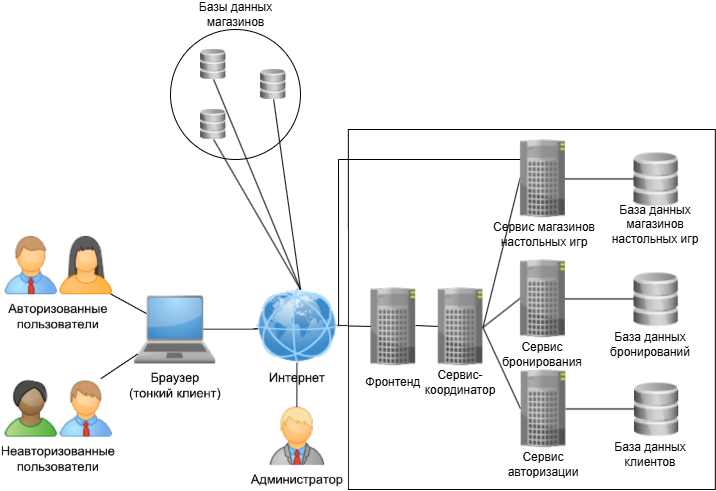
\includegraphics[scale = 0.6]{img/топология.drawio.png}}
		\caption{Топология системы.}
		\label{fig:topology}
	\end{center}
\end{figure}


Система будет состоять из фронтенда и 5 подсистем:
\begin{itemize}
	\item сервис-координатор;
	
	\item сервис регистрации и авторизации;
	
	\item сервис бронирования;
	
	\item сервис оплаты;
	
	\item сервис настольных игр.
\end{itemize}
%
\textbf{Фротенд} принимает запросы от пользователей по протоколу HTTP и анализирует их. На основе проведенного анализа выполняет запросы к микросервисам бекенда, агрегирует ответы и отсылает их пользователю. \\
\textbf{Сервис-координатор} -- единая точка входа и межсервисной коммуникации. \\
\textbf{Сервис-регистрации и авторизации} отвечает за:
\begin{itemize}
	\item возможность регистрации нового клиента;
	
	\item аутентификацию пользователя (клиента и администратора);
	
	\item авторизацию пользователя;
	
	\item выход из сессии.
\end{itemize}
\textbf{Сервис бронирования} отвечает за:
\begin{itemize}
	\item получение, создание бронирования;
	\item создание заявки на отмену бронирования;
	\item изменение статуса заявки бронирования;
	\item изменение статуса бронирования.
\end{itemize}
\textbf{Сервис настольных игр} реализует функции:

\begin{itemize}    
    \item получение списка игр которые есть в наличие в конкретном магазине;
    
    \item получение списка магазинов;
    
    \item добавление нового магазина.
\end{itemize}

\section*{Требования к программной реализации}
\begin{enumerate}
	\item Требуется использовать СОА (сервис-ориентированную архитектуру) для реализации системы.
	
	\item Система состоит из микросервисов. Каждый микросервис отвечает за свою область логики работы приложения и должны быть запущены изолированно друг от друга.
	
	\item При необходимости, каждый сервис имеет своё собственное хранилище,  запросы между базами запрещены.
	
	\item При разработке базы данных необходимо учитывать, что доступ к ней должен осуществляться по протоколу TCP.
	
	\item Необходимо  реализовать  один  web-интерфейс  для  фронтенда.  Интерфейс  должен  быть  доступен  через  тонкий  клиент (браузер).
	
	\item Для межсервисного взаимодействия использовать HTTP (придерживаться RESTful).
	
	\item Выделить Gateway Service как единую точку входа и межсервисной коммуникации. В системе не должно осуществляться горизонтальных запросов.
	
	\item При недоступности систем портала должна осуществляться деградация	функционала или выдача пользователю сообщения об ошибке.
	
	\item Необходимо предусмотреть авторизацию пользователей, как через интерфейс приложения, так и через популярные социальные сети.
	
	\item Проверку правильности входных данных необходимо проводить и на стороне  пользователя,  и  на  стороне  фронтенда. Микросервисы бекенда не должны валидировать входные данные, поскольку пользователь не может к ним обращаться напрямую, они должны получать уже отфильтрованные входные данные.
	
	\item Для запросов, выполняющих обновление данных на нескольких узлах распределенной системы, в случае недоступности одной из систем, необходимо выполнять полный откат транзакции.
	
	\item Приложение должно поддерживать возможность горизонтального и вертикального масштабирования за счет увеличения количества функционирующих узлов и совершенствования технологий реализации компонентов и всей
	архитектуры системы.
	
\end{enumerate}

\section*{Функциональные требования к подсистемам}
Подсистемы: фронтенд, бекенд-координатор, бекенд регистрации и авторизации, бекенд бронирования, бекенд оплаты, бекенд настольных игр.\\
\textbf{Фронтенд} -- серверное  приложение, предоставляет пользовательский интерфейс и внешний API системы, при  разработке которого нужно учитывать следующее:
\begin{itemize}
	\item должен  принимать  запросы  по  протоколу  HTTP и формировать ответы пользователям в формате HTML;
	
	\item в зависимости от типа запроса должен отправлять последовательные запросы в соответствующие микросервисы;
	
	\item запросы к микросервисам необходимо осуществлять по протоколу HTTP;
	
	\item данные необходимо передавать в формате JSON.
\end{itemize}
\textbf{Сервис-координатор} -- серверное приложение, через которое проходит весь поток запросов и ответов, должен соответствовать следующим требованиям разработки:
\begin{itemize}
	\item принимать и возвращать данные в формате JSON по протоколу HTTP;
	
	\item накапливать статистику запросов, в случае, если система не ответила N раз, то в N + 1 раз вместо запроса сразу отдавать fallback. Через некоторое время выполнить запрос к реальной системе, чтобы проверить её состояние;
	
	\item выполнять проверку существования клиента, также регистрацию и аутентификацию пользователей;
	
	\item получение списка всех магазинов с интересующей пользователя игрой в наличии;
	
	\item получение информации и обновление данных о зарегистрированном пользователе;
	
	\item оформление и изменение бронирования;
		
	\item получение данных о бронированиях пользователя;
    
    \item получение, добавление, изменение, удаление детальной информации о магазине;
    
    \item оформление заявки на отмену бронирования.
\end{itemize}
\textbf{Сервис-регистрации и авторизации} должен реализовывать следующие функциональные возможности:
\begin{itemize}
	\item принимать и возвращать данные в формате JSON по протоколу HTTP;
	
	\item возможность регистрации нового клиента и обновление данных уже существующего;
	
	\item проверка существования клиента;
	
	\item обеспечение авторизации пользователя через аккаунт в системе.
\end{itemize}
%
Хранимая в базе данных сущность \textbf{аккаунта}, ассоциированная с сервисом:
\begin{itemize}[label=---]
\item \textit{фамилия}, не более 256 символов;
\item \textit{имя}, не более 256 символов;
\item \textit{отчество}, не более 256 символов;
\item \textit{захешированный пароль};
\item \textit{номер телефона};
\item \textit{электронная почта}, первичный ключ.
\end{itemize}
\textbf{Сервис бронирования} реализует следующие функции:
\begin{itemize}
	\item получение и отправка данных в формате JSON по протоколу HTTP;
	
	\item получение таких данных, как:
	
	\begin{itemize}		
		\item информация о забронированных играх в конкретном магазине;
		
		\item все бронирования, зарегистрированные на конкретного клиента;
		
		\item информация о конкретном бронировании по его идентификатору;
	\end{itemize}
	
	\item составление заявки на отмену бронирования;

	\item создание, редактирование и отмена бронирования.
\end{itemize}
Соответствующая база данных содержит следующую сущность \textbf{бронирования}.
\begin{itemize}[label=---]
\item \textit{идентификатор}, является первичным ключом;
\item \textit{электронная почта клиента};
\item \textit{идентификатор настольной игры};
\item \textit{идентификатор магазина};
\item \textit{статус}, RESERVED/CANCELED/PAID;
\item \textit{дата создания}.
\end{itemize}

Сущность \textbf{заявки на отмену бронирования}.
\begin{itemize}[label=---]
	\item \textit{идентификатор}, является первичным ключом;
	\item \textit{идентификатор бронирования};
	\item \textit{статус}, CREATED/COMPLETED.
\end{itemize}
\textbf{Сервис настольных игр} должен реализовывать представленные такие функциональные возможности, как:
\begin{itemize}
	\item получение и отправка ответов на запросы в формате JSON по протоколу HTTP;
	
	\item получение списка магазинов в которых есть в наличии настольная игра;
	
	\item получение наличия конкретных игр в конкретных магазинах;
	
	\item получение информации о конкретной настольной игре;
	
	\item получение, добавление, изменение, удаление информации о конкретном магазине.
\end{itemize}
Соответствующая база данных содержит следующие сущности.

\begin{enumerate}
	\item \textbf{Магазин}.
	\begin{itemize}[label=---]
		\item \textit{идентификатор}, первичный ключ;
		\item \textit{адрес};
		\item \textit{описание};
		\item \textit{контактная информация}.
	\end{itemize}
\end{enumerate}

\section*{Требования к составу и параметрам технических средств}
Все серверные приложения должны потреблять суммарно не более 4 Гбайт оперативной памяти и работать на сервере с процессором AMD Ryzen 5 4600H 3.00 GHz.

\section*{Требования к надёжности}
Система должна работать в соответствии  с  данным  техническим  заданием  без  рестарта.  Необходимо использовать <<зеркалируемые серверы>> для всех подсистем, которые будут держать нагрузку в случае сбоя до тех пор, пока основной сервер не восстановится.

\section*{Требования к документации}
Исполнитель должен подготовить и передать заказчику руководство:
\begin{itemize}
	\item для Администратора Системы;
	
	\item для Пользователя Системы;
	
	\item для Клиента Системы;
	
	\item по развёртыванию Системы.
\end{itemize}